\chapter{Forms and functions of prosodic prominence} \label{ch:background prominence}

Prominence is a somewhat elusive concept and defining it is notoriously difficult. Many attempts have been put forward, which are often characterized by considerable vagueness and sometimes even contradictoriness \citep{cangemiIntegratingPhoneticsPhonology2020}. Common approaches draw on perception and define prominence in terms of its function. For example, Büring describes prominence as ``a speaker's intuitive sensation of strength in an utterance he or she hears" \citeyearpar[1]{buringIntonationMeaning2016}. Similarly, other definitions reference its ability to make entities \textit{stand out} from their context \citep{terkenFundamentalFrequencyPerceived1991, terkenPerceptionProsodicProminence2000} or \textit{highlight} important information \citep{cangemiIntegratingPhoneticsPhonology2020}. 
	
Two notions that are viewed as central to the concept of prominence in the present book are \textit{relationality} and \textit{redundancy}. As the definitions recited above emphasize, prominent entities stand out from their context by somehow being stronger. These definitions underline the relational aspect of prominence: What is prominent is determined by direct comparison to surrounding entities. An entity that is prominent in one context can even be less prominent than an entity that is considered non-prominent in a different context \citep{cangemiIntegratingPhoneticsPhonology2020}. From an acoustic point of view, this highlighting can be achieved via multiple different prosodic cues related to intonation, timing, and power of the signal \citep[e.g.,][]{fryDurationIntensityPhysical1955, sluijterSpectralBalanceAcoustic1996, kochanskiLoudnessPredictsProminence2005, baumannWhatMakesWord2018, roessigTracingPhoneticSpace2022}. The marking of prominence is thus redundant in nature: When one cue fails or is missing, other cues are available to compensate \citep{winterSpokenLanguageAchieves2014}. Speakers may exploit this redundancy by choosing from the available cues when producing prominence. 

Highlighting or making something stand out can serve multiple pragmatic functions, e.g., marking focus or information status. \citep[e.g.,][]{buringSemanticsIntonationInformation2007, feryPitchAccentScaling2008, baumannCoreferenceLexicalGivenness2013, coleProsodyContextReview2015}. In addition, prosody interacts with syntactic structure. These relations will be explored in more detail in the following sections.

Two clarifying notes on terminology are in order at this point. First, prominence in this book should be understood to refer to \textit{prosodic} prominence unless otherwise specified. This caveat may have been superfluous at one time, however, recent research has advanced the notion of prominence as an organizing principle of language at several levels, including discourse meaning and morphosyntax \citep{himmelmannProminenceProsodyFirst2015, vonheusingerDiscourseProminenceDefinition2019}. Second, prosodic prominence is understood as a post-lexical phenomenon. The term \textit{stress} will be used to refer to word-level ``prominence". 

The following sections will take a closer look at prominence from a formal and a functional perspective. First, Section \ref{section: prominence form} provides an overview of formal aspects of prosodic prominence, both in terms of structural prosodic prominence in the framework of Autosegmental-Metrical Theory (Section \ref{section: structural prominence}) and acoustic correlates of prominence (Section \ref{section: acoustics}). In Section \ref{section: Information structure}, we turn to functional aspects of prominence, specifically information structure marking. Section \ref{section: lexical and syntactic} reports on lexical and syntactic influences on prominence. Finally, Section \ref{section: redundancy} summarizes the previous sections with a view on redundancy and its implications for individual variability in prominence production and perception.

\section{Prosodic prominence: Formal aspects} \label{section: prominence form}

\subsection{Prosodic structure} \label{section: structural prominence}

The present book follows the influential Autosegmental-Metrical (AM) theory of prosody \citep{laddIntonationalPhonology2008}, which builds on the insights of \citet{libermanIntonationalSystemEnglish1975}, \citet{bruceSwedishWordAccents1977}, and \citet{pierrehumbertPhonologyPhoneticsEnglish1980}. Within this framework, prosodic constituents are viewed as hierarchically organized \citep{selkirkPhonologySyntaxRelation1984, hayesProsodicHierarchyMeter1989}. Relevant prosodic layers include the intonation phrase, the intermediate phrase, the prosodic word, and the syllable (see Figure \ref{fig:prosodic_structure}).\footnote{Other potentially relevant layers are the foot or the phonological phrase, which are omitted here for the purpose of simplification without any claim to theoretical adequacy.} The last pitch accent of an intermediate phrase (ip) is considered the nuclear accent \citep[90]{laddIntonationalPhonology2008}, e.g., the pitch accents associated with the words ``cooks" and ``broth" in Figure \ref{fig:prosodic_structure} are nuclear accents in their respective intermediate phrases. The nuclear accent is the only obligatory pitch accent in a phrase and structurally the most important/prominent (\citealt[133, 262-263]{laddIntonationalPhonology2008}, \citealt[3]{calhounCentralityMetricalStructure2010}). However, nuclear accents are not necessarily phonetically the most prominent (\citealt[257]{laddIntonationalPhonology2008}, \citealt[4]{calhounCentralityMetricalStructure2010}). Prenuclear accents, such as the ones associated with ``too" and ``spoil" in Figure \ref{fig:prosodic_structure}, and postnuclear prominences are optional and structurally less prominent than the nuclear accent. Such strength relations between prosodic constituents are captured in the metrical structure, one of the two basic layers of prosody in the AM framework. The second layer is the melody or tune, i.e., the autosegmental tier (\citealt{laddIntonationalPhonology2008, arvanitiAutosegmentalMetricalModelIntonational2022}, see Figure \ref{fig:AM_example}). The two tiers are viewed as independent and orthogonal aspects of intonation \citep[6, 58]{laddIntonationalPhonology2008}. 

\begin{figure}
		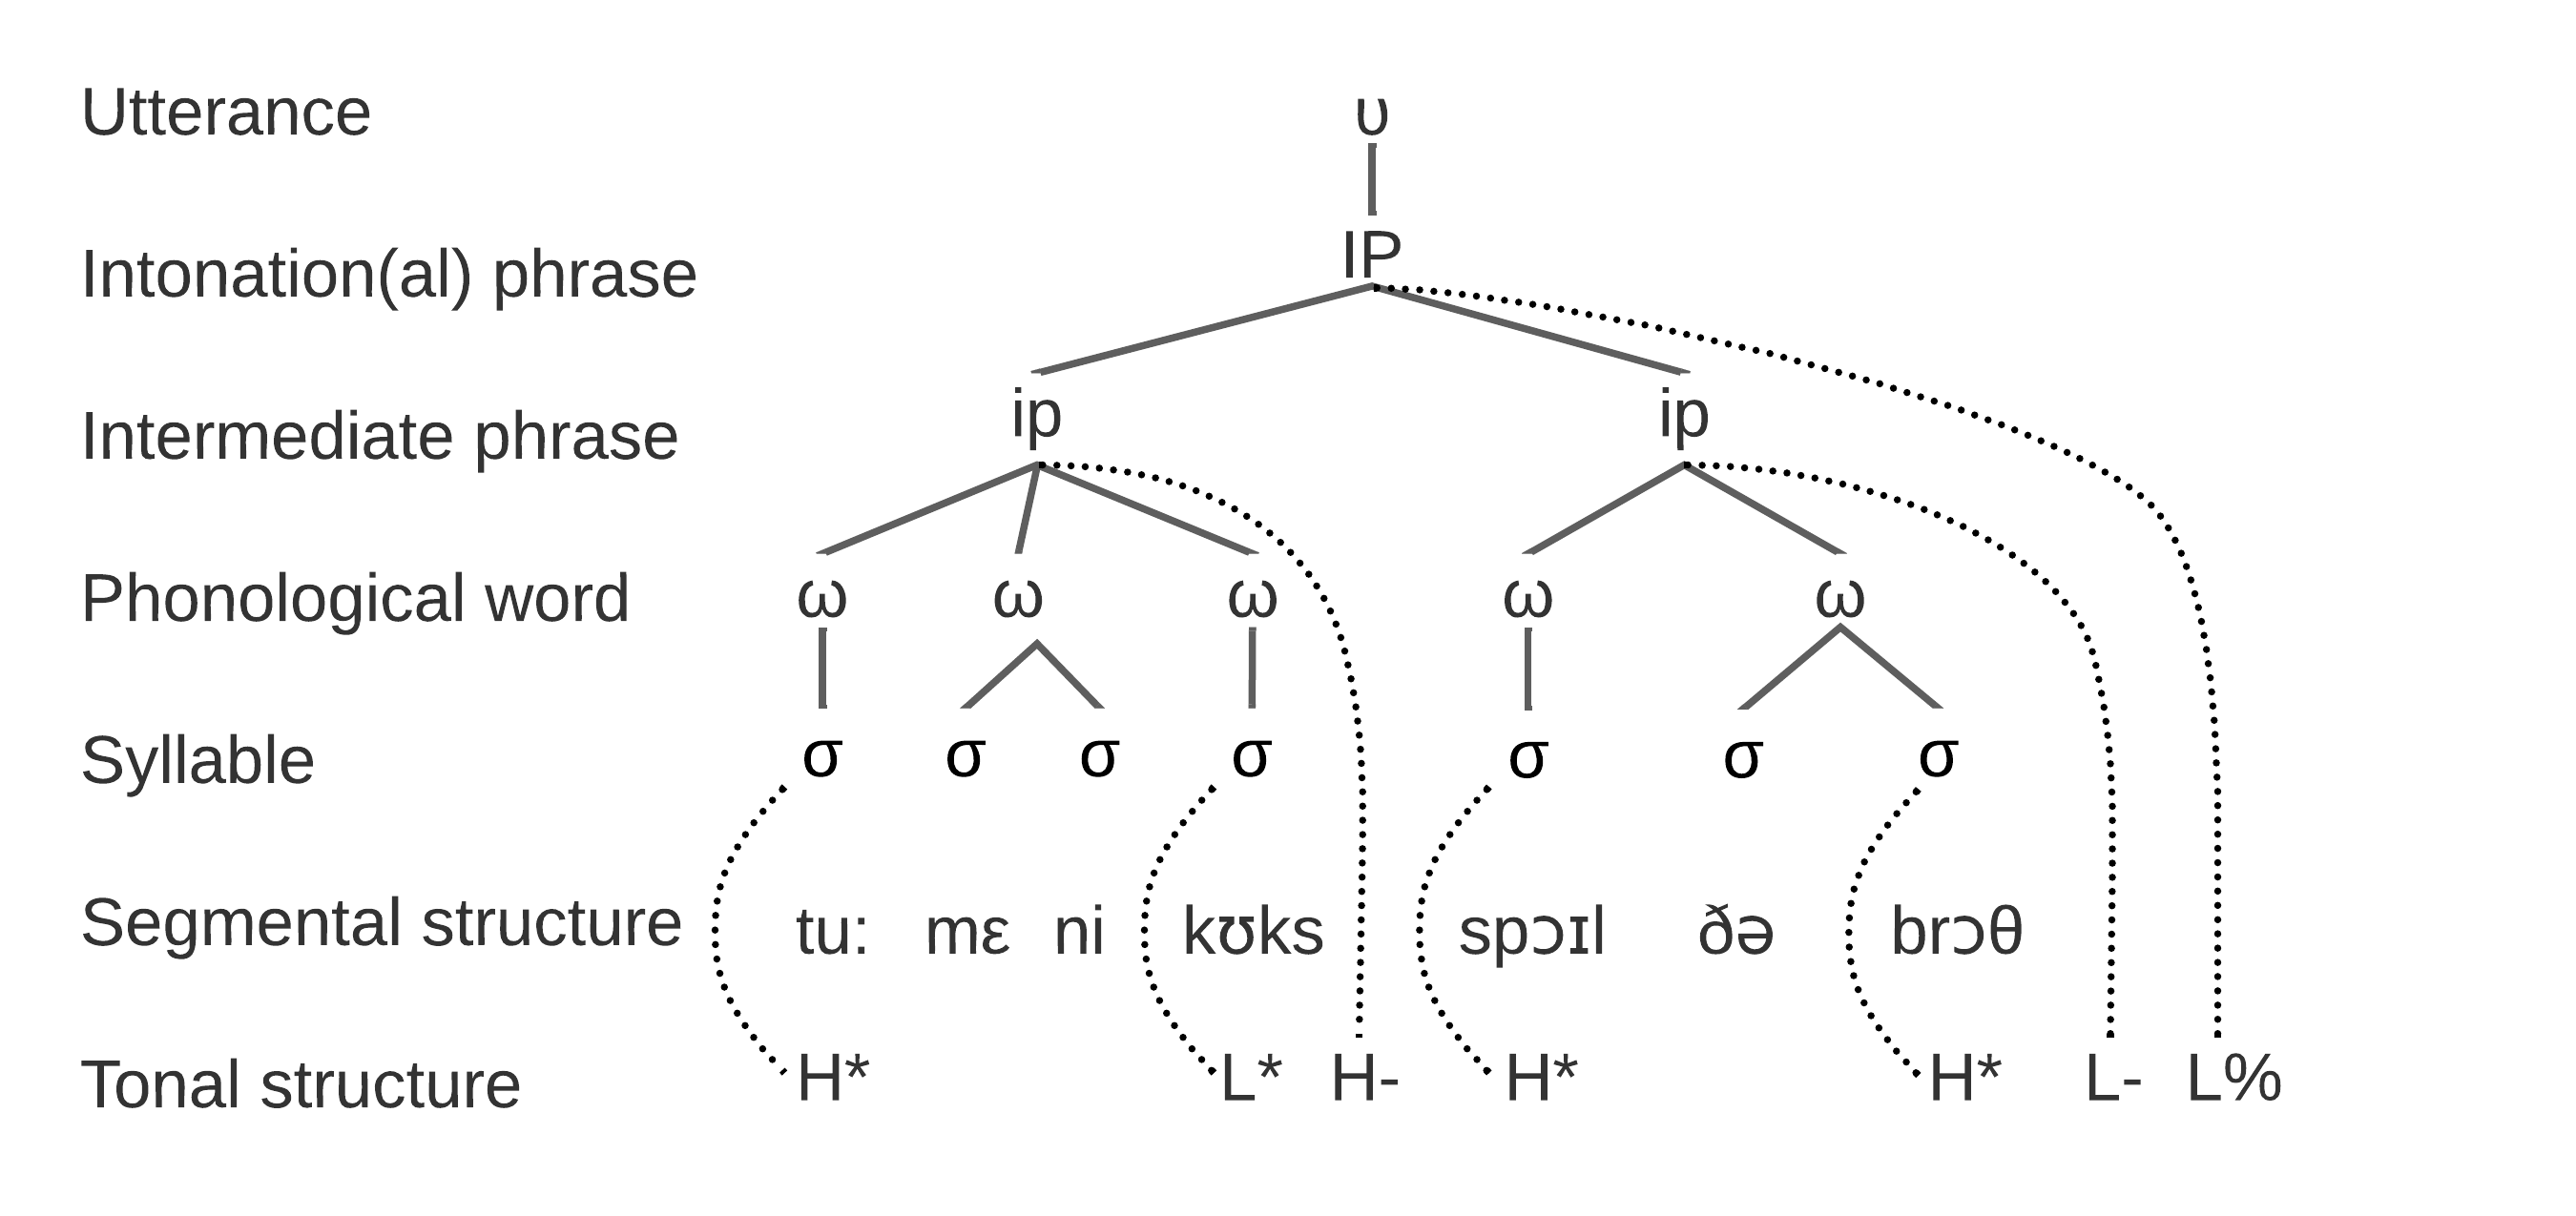
\includegraphics[scale = 0.5]{prosodic structure}
	\caption{Representation of a prosodic hierarchy, exemplified by the utterance ``Too many cooks spoil the broth", adapted from \citet[124]{gussenhovenPhonologyToneIntonation2004} following the reanalysis in \citet[781]{griceIntonation2006}.}
	\label{fig:prosodic_structure}
\end{figure}

In AM, pitch contours are described as sequences of tonal events. In West-Germanic languages, these tonal events encompass pitch accents and edge tones \citep[45]{laddIntonationalPhonology2008}. Intonational pitch accents (as opposed to lexical pitch accents, which occur, for example, in Swedish) are associated with a lexically stressed syllable and cue prominence in that syllable, while edge tones mark the edges of prosodic domains.\footnote{Note that insights from typologically diverse languages caution that assuming a one-to-one mapping between pitch accents and prominence on the one hand and edge tones and phrasing on the other may be too strict an assumption. \citet{griceAutosegmentalmetricalPhonologyUnpacking2022} discusses evidence from three languages that challenge this assumption: First, Tashlhiyt Berber exhibits high peaks that appear to cue prominence but are not associated with a prosodic head and can thus not be analyzed as pitch accents. Second, Maltese has high tones that are associated with a word edge instead of a head, yet also seem to cue prominence. Third, in Bari Italian, postfocal tones may be associated with a head but do not function as cues to prominence.} Between these tonal events, the pitch contour is merely ``transitioning" and thus phonologically unspecified \citep[44]{laddIntonationalPhonology2008}. This is in contrast to a basic assumption of IPO theory (short for \textit{Institute for Perception Research} in Eindhoven, where the IPO theory was advanced, \citealt{thartPerceptualStudyIntonation1990}), in which configurations of the pitch contour are specified that may stretch over several syllables \citep[12, 47]{laddIntonationalPhonology2008}. Tonal events in AM are phonologically specified as either High (H) or Low (L) tones, although the phonetic realization of these tones in terms of pitch scaling is dependent on many factors including emphasis or position in the sentence \citep[44]{laddIntonationalPhonology2008}. Pitch accents may consist of more than one tone and can thus be regarded as configurations, which partially reconciles AM and IPO theories \citep[62-64]{laddIntonationalPhonology2008}.

\begin{figure}
		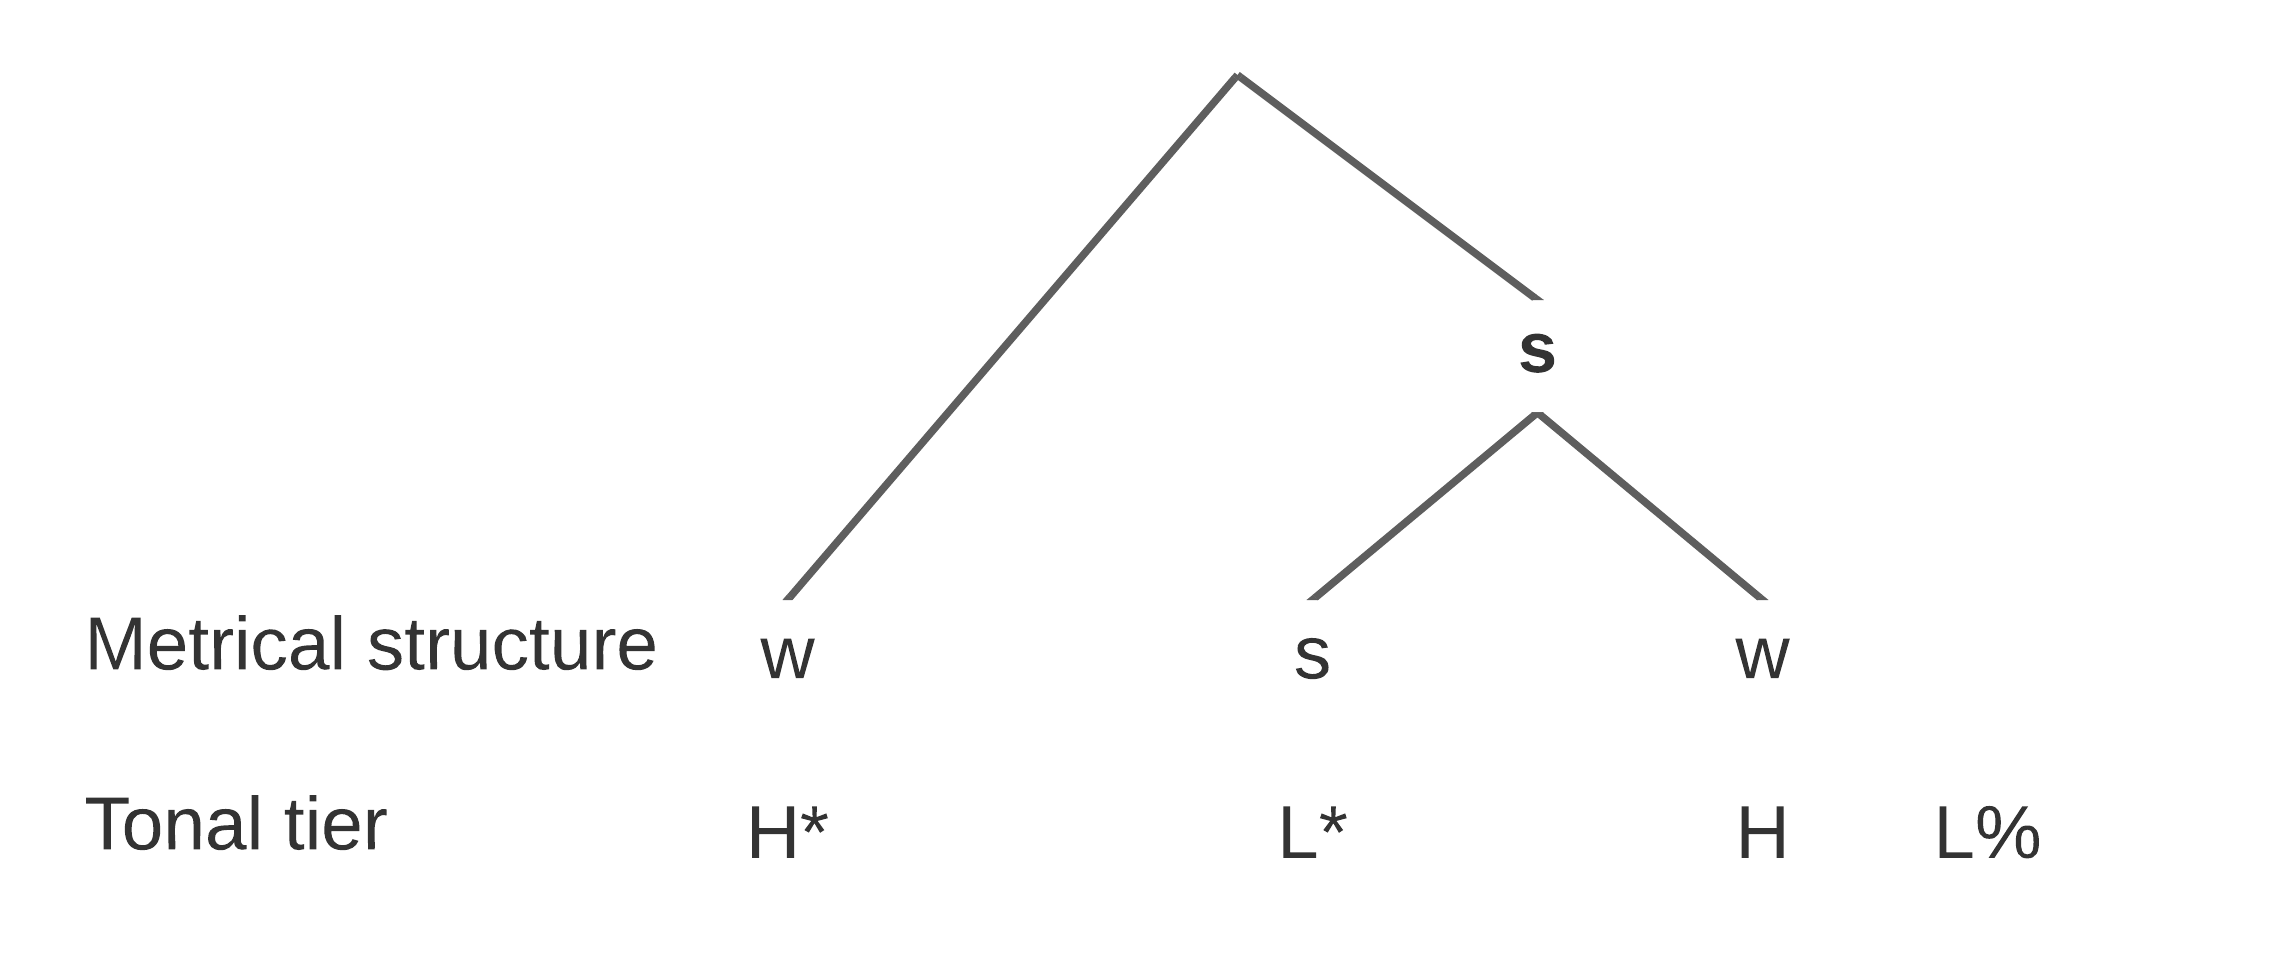
\includegraphics[scale = 0.5]{AM_example}
	\caption{Example of metrical structure and tonal tier in AM, adapted from \citet[284]{laddIntonationalPhonology2008}, representing the Eastern European Question Tune \citep{gricePlacePhraseAccents2000}.}
	\label{fig:AM_example}
\end{figure}

Pitch accents are a manifestation of metrical structure \citep[269]{laddIntonationalPhonology2008}. Metrical structure explicitly pertains to the relational aspect of prominence representing strength relations between the prosodic constituents of an utterance \citep[37]{arvanitiAutosegmentalMetricalModelIntonational2022}. Constituents are specified as strong or weak relative to each other (see Figure \ref{fig:AM_example}). Relationality is thus one of the pillars of AM theory. Crucially, metrical strength relations are understood as abstract and may manifest phonetically in different ways \citep[55-56]{laddIntonationalPhonology2008}. 

Metrical structure has been represented in forms of metrical trees \citep[e.g.,][]{libermanIntonationalSystemEnglish1975} or metrical grids \citep[e.g.,][]{selkirkPhonologySyntaxRelation1984}. In metrical trees, strength relations are represented as binary branching nodes that are labeled strong (s) or weak (w, see Figure \ref{fig:AM_example}). The nuclear accent is dominated exclusively by s-nodes, w-nodes to the left of the nucleus optionally carry a prenuclear accent, nodes to the right may be marked by postnuclear prominences \citep[3]{calhounCentralityMetricalStructure2010}. Metrical trees are by default right-branching, at least in West-Germanic languages, i.e., s-nodes normally occur to the right of w-nodes \citep{libermanIntonationalSystemEnglish1975, laddIntonationalPhonology2008}. Alternatively, in metrical grids, degrees of prominence are formalized in the number of beats assigned to a syllable with the most prominent syllable receiving a beat on a higher metrical level than other syllables \citep[15-16]{selkirkPhonologySyntaxRelation1984}. 

\largerpage
Regarding notation, some conventions have proven useful that are by now relatively widespread: Pitch accents are conventionally marked by stars or asterisks, in bitonal pitch accents, the central tone receives the star \citep[87]{laddIntonationalPhonology2008}. Edge tones can be distinguished by the strength of the prosodic boundary they are associated with. In English, phrase accents (H- or L-) are assumed to mark the end of an intermediate phrase (ip), while boundary tones (H\% and L\%) mark the end of an intonation phrase (IP, \citealt{pierrehumbertPhonologyPhoneticsEnglish1980, beckmanIntonationalStructureJapanese1986}). These conventions are largely followed in AM-based analyses of German intonation \citep[e.g.,][]{feryGermanIntonationalPatterns1993, griceGermanIntonationAutosegmentalMetrical2005}.\footnote{One difference relates to the use of the term \textit{phrase accent}. While in the early American English AM analyses, phrase accents were simply understood as tones marking the boundaries of intermediate phrases, the German system distinguishes between phrase accents that are associated with a postnuclear prominence and phrase tones that mark ip boundaries \citep{griceIntonationLautspracheTonale2016}.} 

Based on Pierrehumbert's \citeyearpar{pierrehumbertPhonologyPhoneticsEnglish1980} work and thereby rooted in the AM tradition, the ToBI (Tones and Breaks Indices) transcription system was introduced by \citet{silvermanTOBIStandardLabeling1992} as an attempt to standardize prosodic annotation. This initiative sprouted many more ToBI systems for a diverse set of languages, among them GToBI for German intonation analysis \citep{griceGermanIntonationAutosegmentalMetrical2005}. GToBI assumes six basic pitch accent types, namely a peak accent H*, a rise from low to peak L+H*, a low accent L*, a valley accent plus rise L*+H, a step-down from high to low H+L*, and a step-down from high to mid H+!H*. Intermediate phrase boundaries are marked by H- or L- tones, intonation phrases additionally by L\% or H\% tones. H tones within pitch accents or boundary tones may also undergo upstep (marked by \textasciicircum) or downstep (marked by !, \citealt[see][67-69 for details]{griceGermanIntonationAutosegmentalMetrical2005}). Break indices, which are used in ToBI annotations to mark boundary strength, play a subordinate role in the GToBI system. In the original ToBI system, four levels of break indices were distinguished, which correspond to very close inter-word junctures (1), phrase-internal word boundaries (2), intermediate phrase boundaries (3), and intonation phrase boundaries (4) \citep{silvermanTOBIStandardLabeling1992, beckmanOriginalToBiSystem2005}. In GToBI, the break indices 3 and 4 still correspond to intermediate and intonation phrase boundaries respectively, however, these break indices are not explicitly annotated beyond the marking of phrase accents and edge tones with the - and \% diacritics. In addition, rhythmic and tonal breaks may be annotated with 2r and 2t respectively to indicate mismatches between tonal and rhythmic structure \citep{griceGermanIntonationAutosegmentalMetrical2005}.

ToBI labeling systems are at their core phonological. From a theoretical perspective, this means that they come with inherent assumptions, e.g., regarding the pitch accent inventory. From a practical side, this can pose difficulties to transcribers, who struggle to make the appropriate phonological abstractions. Theoretical assumptions underlying the ToBI system have been called into question numerous times. For instance, it is a much disputed issue whether L+H* and H* pitch accents should be regarded as two distinct phonological categories or two phonetic realizations of the same category \citep[e.g.,][]{laddIntonationalPhonology2008, arvanitiDisentanglingEmphasisPragmatic2022, laddTroubleToBI2022}. By contrast, there are also suggestions to expand the pitch accent inventory, specifically for German by including an (LH)* accent that phonetically sits between L+H* and L*+H accents (\citealt{zahner-ritterThreeKindsRisingFalling2022}, see also Section \ref{sec:background_F0} for a brief overview of the ``on-ramp versus off-ramp" debate). To resolve practical issues, other labeling systems have been introduced that at least notationally follow the same (AM) tradition but are more phonetic in nature and thus less theoretically loaded. One example is the DIMA annotation system (short for \textit{Deutsche Intonation – Modellierung und Annotation}), which nevertheless adheres to some of the same principles and conventions used in ToBI systems \citep{kuglerDeutscheIntonationModellierung2022}. Similar to these systems, DIMA includes a tonal and a phrasal tier, however, additionally, there is a prominence tier, which allows for the impressionistic annotation of prominence levels independently from the other two tiers. Crucially, DIMA is easier to use for annotators because they need not make phonological abstractions. Nevertheless, DIMA labels are easily translatable into other systems, such as GToBI. 

Specifically, DIMA allows for two types of phrase boundaries to be distinguished, strong (\%) and weak (-). This is similar to GToBI, however, it is cautioned that in DIMA, these boundary types are not directly related to intermediate and intonational phrases in order to remain relatively theory neutral \citep[29]{kuglerDeutscheIntonationModellierung2022}. In terms of tonal annotations, DIMA sticks to the distinction between L and H tones,  allowing especially the H tones to be modified via downstep (!) or upstep (\textasciicircum), similar to GToBI. Three types of tones are distinguished: edge tones, accentual tones, and non-accentual tones. Edge tones mark boundaries, accentual tones are associated with a prominent syllable and marked with a star/an asterisk, and non-accentual tones are turning points that are not prominence-cueing \citep[38]{kuglerDeutscheIntonationModellierung2022}. A difference to GToBI is the treatment of complex labels, such as bitonal pitch accents, which are broken up into their phonetic components, so that each individual label is monotonal. Finally, DIMA adds the prominence tier: Permitted labels are \textit{weak} (1), indicating that a prominent syllable is not necessarily accompanied by F0 movement, \textit{strong} (2), which is typically associated with full pitch accents, and \textit{extra strong} (3), which is used for emphatic realizations of full pitch accents \citep[34]{kuglerDeutscheIntonationModellierung2022}.

Pitch accents, by way of occurring in metrically strong positions, act as a cue to prominence \citep[54]{laddIntonationalPhonology2008}. In addition, multiple continuous measures of the phonetic signal have been investigated as potential correlates of prominence, which are not just related to the pitch contour but also to duration and intensity. The following section summarizes some of the most pervasive findings in this line of research.

\subsection{Acoustic correlates of prominence} \label{section: acoustics}

Prosodic prominence is multidimensional, as it is encoded by a variety of cues related to changes in the fundamental frequency (F0), duration, intensity, and spectral characteristics of the speech signal \citep[e.g.,][]{baumannWhatMakesWord2018, fryDurationIntensityPhysical1955, kochanskiLoudnessPredictsProminence2005, liebermanAcousticCorrelatesWord1960, roessigTracingPhoneticSpace2022, sluijterSpectralBalanceAcoustic1996}. Perceptually, these acoustic cues correspond to pitch, length, and loudness. Generally, prosodically prominent entities are produced with steeper and more rising F0 contours, longer duration, and higher intensity than less prominent entities, at least in West-Germanic languages. There are multiple ways of quantifying each of these acoustic dimensions and since the choice of parameters to be taken as correlates of prominence is crucial for the identification and analysis of individual differences, this section is dedicated to a detailed discussion of the acoustic form of prosodic prominence. The section is divided into the subsections Intonation (\ref{sec:background_F0}), dealing primarily with fundamental frequency, and Timing (\ref{section: timing}), which is concerned with duration and intensity.

\subsubsection{Intonation} \label{sec:background_F0}

Fundamental frequency (F0) has often proven to be the most important correlate of prominence at the phrase-level in West-Germanic languages in general \citep{bolingerTheoryPitchAccent1958, fryExperimentsPerceptionStress1958, liebermanAcousticCorrelatesWord1960, thartPerceptualStudyIntonation1990, bishopPhonologyPhoneticsSignalextrinsic2020, severijnenYourVOORnaamNot2024} and in German in particular \citep{arnoldUsingGeneralizedAdditive2013, niebuhrRelativeCueingPower2017, baumannWhatMakesWord2018, roessigTracingPhoneticSpace2022}. Three characteristics defining the F0 space have been shown to affect (the perceived degree of) prosodic prominence of a syllable or word, namely, (1) the direction of F0 movement, where rising contours are more prominent than falling ones \citep{baumannImportanceTonalCues2014, baumannPerceptualProminencePitch2015}, (2) the height or scaling of the F0 peak, where a higher peak or larger excursion is more prominent than a lower peak \citep{rietveldRelationPitchExcursion1985, laddPerceptionIntonationalEmphasis1997, knightShapeNuclearFalls2008,  baumannPerceptualProminencePitch2015}, and (3) the alignment of the F0 peak with the metrically strong syllable, where a later alignment is more prominent than an earlier one \citep{laddPerceptionIntonationalEmphasis1997, kohlerTimingCommunicativeFunctions2005, niebuhrPerzeptionUndKognitive2007}. 

Numerous operationalizations have been suggested to categorize or quantify these characteristics of the F0 contour. While it is rather straightforward to determine the direction of F0 movement, which can only ever be rising, falling or level, there are substantial methodological differences in capturing the extent of the rise or fall, i.e., F0 scaling as well as alignment, which are intertwined with underlying theoretical considerations. Major differences between such operationalizations are whether they take a categorical or a continuous approach, whether they rely on annotated landmarks, such as F0 minima or maxima and turning points, or derive directly from the (weighted) signal and whether they combine several of the aforementioned F0 characteristics or single out only one of them.

One popular approach to categorizing the F0 contour, especially the part that aligns with metrically strong syllables, is via the aforementioned prosodic annotation schemes ToBI for American English \citep{silvermanTOBIStandardLabeling1992,beckmanOriginalToBiSystem2005} and GToBI for German \citep{griceConsistencyTranscriptionLabelling1996, griceDeutscheIntonationUnd2002}. Pitch accents defined as ``pitch movements or configurations that lend prominence to their associated word" \citep[868]{silvermanTOBIStandardLabeling1992} can be understood as bundles of acoustic cues that are identified and labeled as they are perceived by a listener (i.e., the annotator). Classifying the type of pitch accent requires consideration of direction of movement (e.g., L+H* marks a rising accent, H+!H* a falling one), scaling (L* is defined as a low accent, H* as a high accent), and alignment (L*+H describes a low target on the accented syllable followed by a rise, L+H* indicates that a high target is already reached within the accented syllable, \citealt[see][]{griceGermanIntonationAutosegmentalMetrical2005}). Since the annotator bases their decision on a holistic impression of the signal, such categorizations involve the perception of changes in duration or intensity in addition to pitch. The GToBI guidelines even explicitly note that intensity and duration may be decisive when annotating L* accents \citep[278]{baumannImportanceTonalCues2014, griceDeutscheIntonationUnd2002} as the difference between an L* accented and an unaccented syllable may be one of perceived length and loudness in the absence of a noticeable pitch movement. 

While the presence of a pitch accent already indicates higher prominence relative to a lack of pitch accent, accent types can further be ordered by their (perceived) degree of prominence. \citet{baumannPerceptualProminencePitch2015} showed that for German, the following hierarchy in terms of perceived prominence (left to right from most prominent to least prominent) emerges: 

\hspace*{20mm}L+H* > L*+H > H* > H+!H* > H+L* > !H* > L*

What becomes apparent from this ranking is that the direction of pitch movement is most important for the perception of prominence, with rising contours being judged as more prominent than falling ones. However, scaling also plays a role, both in absolute terms, in that high accents are more prominent than low accents and considering more dynamic changes, in that accents including larger pitch movement (e.g., H+!H* and H+L*) are more prominent than relatively level accents (e.g., !H* and L*). \citet{baumannWhatMakesWord2018} confirm these findings albeit using broader accent type categories, with rising accent types being judged as most prominent followed by high, falling, and low accents, respectively. A similar ranking of accent types in terms of perceived prominence was established by \citet{bishopPhonologyPhoneticsSignalextrinsic2020} for American English.
 
When considering accent type as a correlate of prosodic prominence, it comes as no surprise that a variable involving several acoustic dimensions is a more robust correlate of prominence than an isolated cue, such as mean or maximum F0. \citet{baumannWhatMakesWord2018} showed that categorical prosodic variables, e.g., accentedness (i.e., the presence or absence of a pitch accent) and type of pitch accent, were more predictive of perceived prominence than continuous variables. A similar conclusion is reached by \citet{bishopPhonologyPhoneticsSignalextrinsic2020}. However, there is some criticism surrounding the ToBI system in particular (see Section \ref{section: structural prominence} for some arguments) and the use of categorizations of the pitch contour in general. For example, \citet{griceIntegratingDiscretenessContinuity2017} investigating continuous and categorical prosodic correlates of different focus types in German found that although not all speakers make categorical distinctions in terms of pitch accent type between different focus types, listeners are still able to derive the correct intended function. They conclude that ``discrete pitch accent categories are only a poor approximation for how listeners comprehend intended pragmatic meanings" \citep[101, see Section \ref{section: Information structure} for a more detailed discussion of the prosodic encoding of meaning contrasts]{griceIntegratingDiscretenessContinuity2017}. In a similar vein, \citet{laddTroubleToBI2022} cautions that overly relying on categories may result in the neglect of meaningful gradient variation. 

This issue is immediately relevant to the present book as coarse-grained categorization may also gloss over individual variability. For example, \citet{niebuhrAreThereShapers2011} observed that German speakers differed in whether they relied on F0 shape or alignment in order to distinguish between H* and H+L* accents. In order to arrive at a better understanding of the nature of individual variability, it is thus necessary to consider gradience in the prosodic signal by looking at continuous operationalizations of acoustic parameters.

Theoretical assumptions shaping prosodic classification systems also have implications for considerations regarding continuous measures. One major point of contention has been the on-ramp versus off-ramp debate \citep[see][]{gussenhovenPhonologyToneIntonation2004, ritterRoleTonalOnglides2015, barnesRampsIntonationalPhonology2021}. In an on-ramp approach, the nuclear tone and the movement \textit{towards} it are considered most important for the interpretation of an F0 contour, while conversely, in an off-ramp model, the nuclear tone and the movement \textit{away from} it are considered decisive. Systems devised in the tradition of the British school are considered off-ramp approaches \citep[e.g.,][]{gussenhovenTranscriptionDutchIntonation2005, petersPhonologicalSemanticAspects2018}, ToBI annotation systems, such as the classic Mainstream American English ToBI \citep{silvermanTOBIStandardLabeling1992,beckmanOriginalToBiSystem2005} and the German GToBI \citep{griceConsistencyTranscriptionLabelling1996, griceDeutscheIntonationUnd2002}, can be regarded as predominantly on-ramp approaches. However, such classifications are not completely definitive as, for instance, the GToBI inventory also includes an L*+H accent, which describes a pitch accent in terms of its nuclear and trailing tone. When quantifying the F0 curve in a continuous measure, for example with regard to excursion size, one similarly has to make the theoretical decision whether to consider the tonal onglide, the offglide, or both. There is, in fact, empirical evidence to support both approaches. In a perception study, \citet{ritterRoleTonalOnglides2015} found that German listeners were able to make use of tonal onglide in order to determine if an utterance contained given/non-contrastive or new/contrastive information. Similarly, \citet{braunPrenuclearActivatesAlternatives2019} found that the F0 contour leading up to and including the accented syllable was particularly important for German listeners' interpretation of utterances with regard to their contrastiveness. In contrast, \citet{barnesRampsIntonationalPhonology2021} found that American English listeners relied on tonal onglide and offglide to an almost equal extent, at least when it comes to tonal events ranging from contours typically defined as H+!H* to L+H*. However, when looking at a continuum of values typical of L*+H to L+H* accents, the shape of the fall seemed to matter much less than the shape of the rise. Taken together, these findings suggest that it may be more important to account for the on-ramp in order to accurately describe prosodic prominence.

Oftentimes, continuous measures rely on (annotated) landmarks or turning points in the F0 contour or average across certain parts of the signal. Such measures can be quite successful at capturing prominence, for example, in \citet{roessigTracingPhoneticSpace2022}, where only continuous parameters were considered, mean F0 was the most important correlate to distinguish accented from unaccented words, outperforming measures accounting for aspects of duration, intensity, formant values, and articulatory gestures. However, concerns have been raised that these landmarks determined by the peaks and elbows in the continuous F0 trajectory may not accurately reflect perceptual reality \citep{albertModelSonorityBased2023} and that static parameters calculated from these landmarks (e.g., peak alignment, pitch excursion, or tonal onglide) may conceal more fine-grained information, such as pitch accent shape \citep{barnesTonalCenterGravity2012}. To address these issues, more sophisticated measures have recently been proposed. 

One such measure of F0, which takes into account both the shape of the rise and the shape of the fall of an accent and thus also unifies on-ramp and off-ramp approaches, is the Tonal Center of Gravity (TCoG, \citealt[see][]{barnesTonalCenterGravity2012, barnesRampsIntonationalPhonology2021}). The TCoG measures represent an alternative to traditional measures that are reliant on turning points and are able to capture both alignment in time and F0 scaling (see Figure \ref{fig:TCoG}). TCoG alignment (or TCoG-t) constitutes a point in time relative to the beginning of the target domain weighted by the F0 contour. Values of TCoG alignment are higher the later a rise occurs and the more \textit{scooped} the F0 contour. Conversely, values are lower the earlier the rise and the more \textit{domed} the F0 shape. TCoG alignment thus more closely captures \textit{perceived} alignment, which is not only influenced by actual peak alignment but also by the shape of the F0 movement surrounding the peak \citep{barnesTonalCenterGravity2012}. TCoG scaling (or TCoG-f) is measured as the weighted average F0 over the target domain. Crucially, more sonorous regions contribute more to the value of TCoG scaling, as it is assumed that F0 in these regions is more salient to the listener \citep{barnesSegmentalInfluencesPerception2014}. 

\begin{figure}
		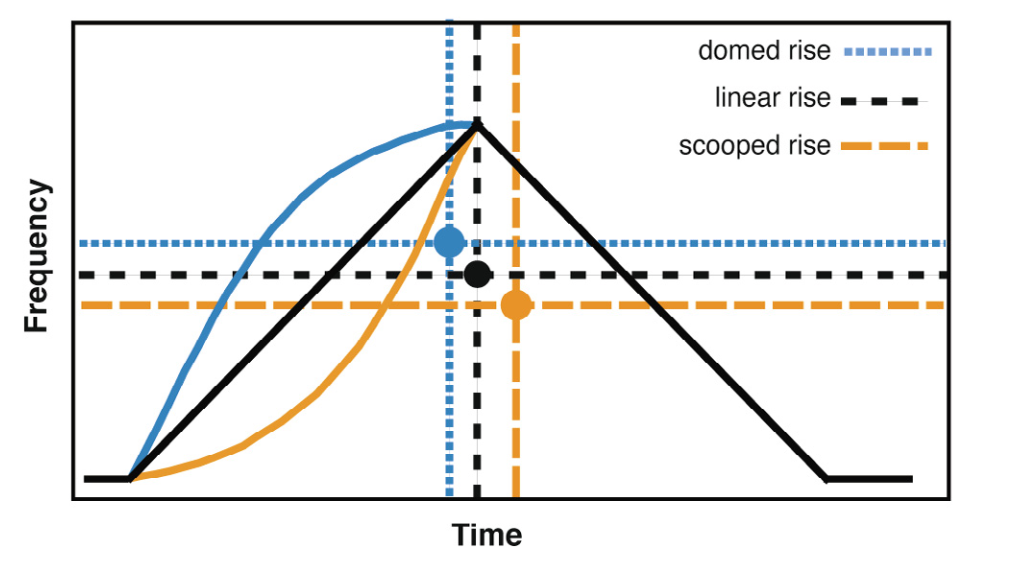
\includegraphics[scale = 0.2]{TCoG}
	\caption{Schematization of TCoG alignment and scaling \citep[6]{barnesRampsIntonationalPhonology2021}. A \textit{domed} F0 contour leads to an earlier and higher TCoG (colored circles), a \textit{scooped} contour to a later and lower TCoG.}
	\label{fig:TCoG}
\end{figure}

TCoG measures thus quantify information about the F0 contour shape that is not captured by traditional measures of scaling and alignment and has been shown to more accurately describe prosodic phenomena in some studies. For instance, TCoG alignment more robustly distinguished between L*+H and L+H* pitch accents in American English productions than traditional turning point alignment values \citep{barnesTonalCenterGravity2012}. Results from a study by \citet{bruggemanUnifyingSpeakerVariability2017} also favor TCoG (alignment) over turning point based measures of alignment and scaling, as the former yields a more unified picture of focus type marking in Egyptian Arabic across different speakers. Analogously to traditional measures of alignment and scaling, a higher TCoG alignment value (i.e., later alignment of the bulk of the F0 contour) and higher TCoG scaling is assumed to correlate with a higher degree of prominence. 

Another recent suite of prosodic measurements, which was partly inspired by \citeauthor{barnesTonalCenterGravity2012}'s \citeyearpar{barnesTonalCenterGravity2012} Tonal Center of Gravity, comes from the ProPer toolbox \citep{albertUsingPeriodicEnergy2018, albertModelSonorityBased2023}. ProPer stands for PROsodic analysis with PERiodic energy and has its origins in research on sonority \citep{albertModelSonorityBased2023}. Periodic energy, which is the log transform of the acoustic power in the periodic parts of the signal (see \citealt[143-145]{albertModelSonorityBased2023} for details), is taken as the acoustic correlate of sonority. Fluctuations in the periodic energy curve thus correlate systematically with syllable boundaries. Perceptually, periodic energy also links to pitch intelligibility \citep[55-56]{albertModelSonorityBased2023}, which is presumably enhanced in portions of the signal produced with higher periodic energy (see Figure \ref{fig:proper_simple}). ProPer thus combines several acoustic dimensions to derive acoustic measurements that are firmly grounded in perceptual reality, making it the most suitable toolbox for the present investigation. 

\begin{figure}
		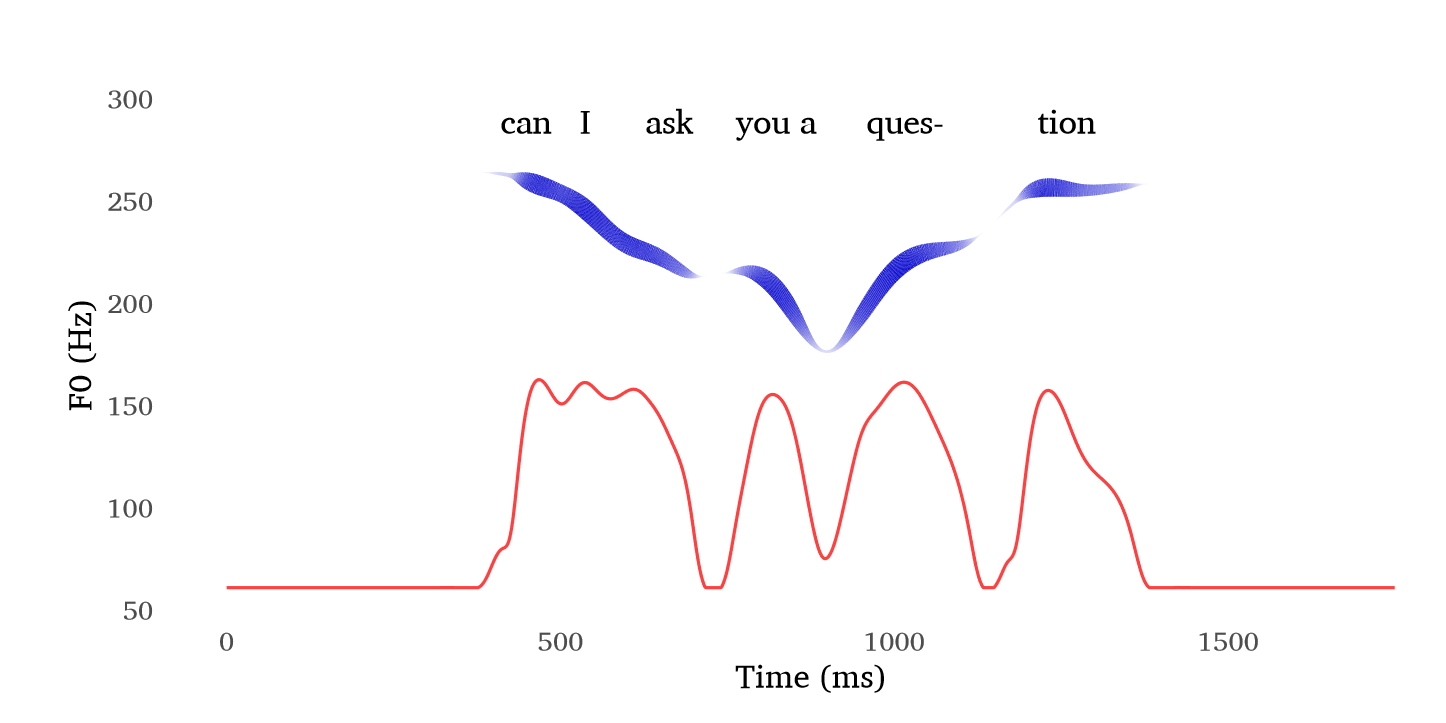
\includegraphics[scale = 0.2]{proper}
	\caption{Schematization of the relation between F0 curve (blue) and periodic energy (red), i.e., a ``periogram" \citep[153]{albertModelSonorityBased2023}. Note that the F0 curve is enhanced by periodic energy, that is, it is thicker in areas with higher periodic energy as indicated by the red curve. The y-axis on the left corresponds only to the F0 curve, not to periodic energy.}
	\label{fig:proper_simple}
\end{figure}

Based on the periodic energy curve (Figure \ref{fig:proper_simple}, red line) and the F0 curve modulated by periodic energy (Figure \ref{fig:proper_simple}, blue line), a number of prosodic variables can be computed, which correspond to cues that are traditionally assumed to correlate with prosodic prominence, such as F0 alignment and scaling. Methodologically, similar to TCoG, this has the advantage that there is no need for prior labeling of turning points. Instead, points of interest are directly computed from the signal. Specifically, for each syllable, a Center of Mass (CoM) and a Center of Gravity (CoG) can be determined. The CoM is the point in time that splits the area under the periodic energy curve of a syllable into two equal parts. Measuring the F0 at the CoM yields a robust representation of perceived peak height, which roughly corresponds to TCoG scaling (TCoG-f). A Delta F0 value can be calculated by measuring the F0 at the CoM of two subsequent syllables and taking their difference. Delta F0 thus constitutes a measure of the extent and direction of F0 change across syllables, which can be interpreted similarly to tonal onglide or tonal offglide, depending on which syllables are being compared. Analogous to the TCoG by \citet{barnesTonalCenterGravity2012, barnesRampsIntonationalPhonology2021}, in the ProPer framework, a Center of Gravity (CoG) is computed as an averaged point in time weighted by the F0 curve multiplied by periodic energy. CoG can thus be used as a measure replacing traditional F0 peak alignment or TCoG alignment. Relating the distance between the CoM and the CoG yields another ProPer measure, namely synchrony. Synchrony accounts for the extent and direction of F0 change within one syllable as well as the contour's shape. If the CoG is located to the right of the CoM (reflected in a positive synchrony value), F0 is rising within the syllable, if the CoG occurs to the left of the CoM (synchrony is negative), F0 is falling. If CoG and CoM are perfectly aligned (i.e., synchrony has a value of 0), the F0 contour is either level or exhibits a symmetrical rise-fall or fall-rise.

Although initially designed for the study of sonority, ProPer measures have proven useful in quantifying prominence phenomena as well \citep{roessigTracingPhoneticSpace2022, sbrannaProsodicMarkingInformation2023}. For example, \citet{roessigTracingPhoneticSpace2022} found synchrony to successfully distinguish broad from narrow and contrastive focus domains as well as narrow from contrastive focus in German, with higher synchrony indicating higher prominence.

\subsubsection{Timing} \label{section: timing}

Further gradient prosodic cues capturing the acoustic dimensions of duration and intensity have been found to be related to prominence in production and perception. These are jointly considered here under the notion of timing, since both dimensions contribute to a perception of rhythm in speech \citep[cf.][]{albertRhythmTimescale2024}. Numerous studies have shown that more prominent units are produced with longer duration and higher intensity than less prominent units and that longer and louder units are perceived as being more prominent (e.g., \citealt{fryDurationIntensityPhysical1955, beckmanStressNonStressAccent1986, aylettSmoothSignalRedundancy2004,  coleSoundStructureMeaning2019}). In terms of a ranking of prominence correlates, Fry's \citeyearpar{fryDurationIntensityPhysical1955, fryExperimentsPerceptionStress1958} perceptual studies suggest that duration ranks higher than intensity but lower than F0 in cueing prominence for American English listeners. Similarly, \citet{turkProcessingDurationIntensity1996} find duration to be more important to the perception of prominence and intensity independent of duration to contribute little to the perception of prominence. However, in their production study on German, \citet{roessigTracingPhoneticSpace2022} find that intensity (measured as RMS amplitude) is more successful than vowel duration in distinguishing accented from unaccented words. Intensity is also found a better predictor to prominence than duration in \citet{liebermanAcousticCorrelatesWord1960} and \citet{kochanskiLoudnessPredictsProminence2005}. These differences may stem from different manipulations of the speech material under investigation or from different operationalizations of the duration and intensity measures.

Measuring duration is primarily a matter of determining segmental boundaries, but studies differ in which domain they consider for their duration measurement. Common choices (all including the syllablic nucleus) are the vowel \citep[e.g.,][]{fryDurationIntensityPhysical1955, beckmanStressNonStressAccent1986, turnbullListenerorientedPhoneticReduction2019, roessigTracingPhoneticSpace2022}, the syllable \citep[e.g.,][]{aylettSmoothSignalRedundancy2004, baumannTonalArticulatoryMarking2007, muckeEffectFocusMarking2014}, the foot \citep{baumannTonalArticulatoryMarking2007, muckeEffectFocusMarking2014}, and the word \citep[e.g.,][]{bakerVariabilityWordDuration2009, breenAcousticCorrelatesInformation2010, coleSoundStructureMeaning2019, turnbullListenerorientedPhoneticReduction2019}. In \citet{muckeEffectFocusMarking2014}, syllable and foot (which is equivalent to the word domain in their study) duration are similarly effective in distinguishing between different focus types. \citet{baumannTonalArticulatoryMarking2007}, however, found that focus types may be more robustly encoded in the duration of the foot than that of the syllable. \citet{turnbullListenerorientedPhoneticReduction2019} observed that unpredictability is marked by both longer vowel duration and longer word duration, but that individual speakers differed in the extent to which they manipulated these two variables. The question of which duration measure is optimal to capture prominence effects is thus not yet conclusively determined and it may be beneficial to consider duration over both a smaller domain (such as the syllable) and a larger domain (such as the word).

Intensity can also be quantified in various ways. Traditionally, studies consider either peak or mean overall intensity \citep[e.g.,][]{fryDurationIntensityPhysical1955} measured as the sound pressure level or RMS amplitude over the full spectrum. However, since the seminal study by \citet{sluijterSpectralBalanceAcoustic1996}, newer measures have gained popularity that calculate the intensity in or intensity ratios across parts of the spectrum, i.e., the spectral emphasis, spectral balance or spectral tilt/slope. This approach is motivated by the perceptual correlate of intensity, which is loudness. \citet{sluijterSpectralBalanceAcoustic1996} argue that intensity in lower frequencies (up to 500 Hz) contribute less to perceived loudness than intensity in higher frequencies. Indeed, \citet{sluijterSpectralBalanceAcoustic1996} found that what they call spectral balance is a better correlate of lexical stress than intensity. Although the study by \citet{sluijterSpectralBalanceAcoustic1996} was concerned with the acoustic correlates of lexical stress, this relation between spectral balance and loudness should generally hold true and thus extend to phrase-level prominence. In fact, \citet{heldnerSpectralEmphasisAdditional2001} found spectral emphasis to outperform overall intensity in classifying phrase-level accent in Swedish.

However, in contrast to findings by \citet{sluijterSpectralBalanceAcoustic1996} and \citet{heldnerSpectralEmphasisAdditional2001}, \citet{kochanskiLoudnessPredictsProminence2005} in their study using classifiers trained on human prominence judgments found that overall intensity by far outperformed spectral slope in distinguishing prominent from non-prominent syllables. Such differing findings may again arise from different operationalizations. As already apparent from the terminological chaos, there are many ways to measure spectral emphasis, slope, balance or tilt. \citet{heldnerReliabilityOverallIntensity2003} provides a brief overview of different measures and terminology. He suggests a broad binary distinction between spectral tilt and spectral emphasis, the former measuring the slope of the spectrum and the latter relative energy in higher-frequency bands \citep[40]{heldnerReliabilityOverallIntensity2003}. However, within these two categories, several more fine-grained distinctions can be made and there is no consensus on the best way to obtain these measures. In summary, it seems that spectral balance and spectral emphasis are not (much) more successful in capturing prominence at a phrasal level than overall intensity \citep{sluijterSpectralBalanceAcoustic1996, heldnerSpectralEmphasisAdditional2001, kochanskiLoudnessPredictsProminence2005}, which is also easier to obtain. 

Some research suggests that duration and intensity may be processed together \citep[e.g.,][]{turkProcessingDurationIntensity1996}. This justifies a measure combining these two acoustic dimensions, such as periodic energy mass \citep{albertModelSonorityBased2023}. Periodic energy mass quantifies the area under the periodic energy curve within an interval, i.e., the syllable. It is the integral of duration and power. \citet{roessigTracingPhoneticSpace2022} found periodic energy mass to be among the most important prosodic cues to distinguish accented from unaccented words. Similarly, in \citet{sbrannaProsodicMarkingInformation2023}, periodic energy mass was the most important correlate of marking information status in Italian.

To summarize, prosodic prominence relates to multiple acoustic dimensions that can each be measured or categorized in various ways, which has implications for findings regarding their robustness and strength. The present book draws from categorical and continuous approaches to prosody, while reducing the number of prosodic parameters under consideration to a reasonable number (see Sections \ref{section: measurements study1} and \ref{section: measurements study2} for details). The following sections will now explore prosodic prominence from a functional perspective.

\section{Information structure and prosodic prominence} \label{section: Information structure}

One of the functions of prosodic prominence is marking information structural categories, such as focus and information status. Information structure encompasses several theoretical concepts, such as the distinctions between focus and background, theme and rheme, topic and comment, as well as givenness and newness. \citet[199]{hallidayNotesTransitivityTheme1967} defines information structure as ``the relation of what is being said to what has gone before in the discourse" and the ``internal organization [of a clause] into an act of communication." Information structure is thus related to the communicative function of managing common ground \citep[e.g.,][]{krifkaBasicNotionsInformation2008}. This chapter will unpack the notions of focus and givenness (or information status) and their relation to prosodic prominence. The latter are discussed with regard to West-Germanic languages in particular, as the mapping of prosody to information structure is far from universal and other languages may rely predominantly on non-prosodic factors, such as word order or morphological focus particles \citep[e.g.,][]{buringTypologyFocusRealization2009}. As far as information structural categories are concerned, information status is the primary interest of the present book. However, since focus is intricately linked with information status and much prosodic research has been dedicated to the study of focus marking, the following sections will introduce and attempt to disambiguate both concepts. 

\subsection{Focus} \label{sec: focus background}

One of the most important information structural categories is that of focus. \citet[204]{hallidayNotesTransitivityTheme1967} suggests that information \textit{in focus} is presented by the speaker ``as not being recoverable from the preceding discourse." Similarly, \citet[448]{buringSemanticsIntonationInformation2007} argues that focus occurs in conjunction with the most informative part of a sentence. \textit{Background} is generally used as a complementary notion to focus: What is not in focus is in the background. A well-established idea of focus from the theory of Alternative Semantics defines focus by its property of introducing a set of alternatives \citep{roothTheoryFocusInterpretation1992}. These alternatives are relevant for the interpretation of the focused expression \citep[see also][]{krifkaBasicNotionsInformation2008}. In example \ref{itm:Mona}, the focused entity is ``Mona", marked by square brackets and a subscript \textsubscript{F}. The expression ``Mona" induces a set of alternatives, i.e., people who broke their arm. ``Mona" also corresponds to the wh-expression in the preceding question. This correspondence is known as Question-Answer Congruence and can serve as a tool to identify the focus domain \citep[e.g.,][]{buringSemanticsIntonationInformation2007}. 

\begin{enumerate}[label=(\arabic*)]
\item \label{itm:Mona} Who broke their arm?\newline[MOna]\textsubscript{F} broke her arm.
\end{enumerate}

Focused parts of an utterance are prosodically emphasized, i.e., produced with a pitch accent \citep[e.g.,][]{hallidayNotesTransitivityTheme1967, cutlerSemanticFocusSentence1979}. Specifically, the nuclear accent has a special role in signaling focus \citep[257, 259]{laddIntonationalPhonology2008}. In example \ref{itm:Mona} above, the nuclear accent falls on the first syllable of ``Mona" (as signaled by capitalization) marking ``Mona" as the focused constituent, while the rest of the sentence is deaccented and in the background. Under the Focus-to-Accent approach \citep[e.g.,][]{hallidayNotesTransitivityTheme1967, gussenhovenFocusModeNucleus1983, selkirkPhonologySyntaxRelation1984}, the location of the nuclear accent follows logically from language-specific rules once the focus domain is known. Conversely, the location of the nucleus indicates which constituent is in focus. However, it is not necessarily just the pitch accented constituent that is in focus. In the case of broad focus, the pitch accent is assumed to \textit{project} focus onto a larger prosodic constituent as in example \ref{itm:house}, where the focus domain encompasses the complete sentence \citep{selkirkPhonologySyntaxRelation1984, selkirkSentenceProsodyIntonation1995}. The constituent receiving the nuclear accent, e.g., ``house" in the present example, is the focus exponent \citep{laddIntonationalPhonology2008}.

\begin{enumerate}[resume*]
\item \label{itm:house} What happened?\newline
[Lola sold her HOUSE.]\textsubscript{F}
\end{enumerate}

Types of focus can thus be distinguished by their scope: Example \ref{itm:Mona} is an instance of narrow focus, example \ref{itm:house} represents broad focus. Additionally, focus has been classified by the degree of contrastiveness that is evoked \citep{laddStructureIntonationalMeaning1980, laddIntonationalPhonology2008}. \citet{calhounCentralityMetricalStructure2010} following \citet{bolingerFormsEnglishAccent1965} argues that all focused entities induce some contrast by way of introducing a set of alternatives. The degree of contrastiveness is a matter of the restrictedness of the number of alternatives \citep[8]{calhounCentralityMetricalStructure2010}. In broad focus, the set of alternatives is not clearly defined \citep[8]{calhounCentralityMetricalStructure2010}. The highest degree of contrastiveness is induced in corrective focus \citep{gussenhovenPhonologyToneIntonation2004}, where the focused constituent presents a direct alternative to a previously established entity as in example \ref{itm:horse}, where ``house" contrasts with ``horse".

\begin{enumerate}[resume*]
\item \label{itm:horse} Did Lola sell her horse?\\
Lola sold her [HOUSE.]\textsubscript{F}
\end{enumerate}

The relation between focus (types) and prosodic prominence in West-Germa\-nic languages has received much attention in recent research \citep[e.g.,][]{feryPitchAccentScaling2008, muckeEffectFocusMarking2014, roessigTracingPhoneticSpace2022}. Studies have identified both categorical and continuous correlates of focus in addition to accentuation patterns. Several studies observed a probabilistic mapping of focus type and accent type in German. For example, \citet{baumannTonalArticulatoryMarking2007} found that !H* accents were more common in broad focus, while contrastive focus was often produced with \textasciicircum H* accents. Similarly, in data presented by \citet{muckeEffectFocusMarking2014} and \citet{griceIntegratingDiscretenessContinuity2017}, speakers produced mostly falling accents (H+!H*) in the broad focus condition, while an L+H* accent was preferred in contrastive focus. Crucially, more prominent accent types \citep[according to the hierarchy presented in][]{baumannPerceptualProminencePitch2015} are more frequent the more contrastive the focus.

In addition, studies have found several continuous prosodic cues to focus. For example, \citet{griceIntegratingDiscretenessContinuity2017} observed earlier peak alignment in broad focus and later alignment in contrastive focus with narrow focus in between as well as smaller tonal onglide values in broad focus than in narrow and contrastive focus. Accordingly, rising onglides were also more likely to be perceived as signaling new/contrastive information and falling onglides to signal given/non-con\-tras\-tive information in \citet{ritterRoleTonalOnglides2015}. In line with these findings, \citet{roessigTracingPhoneticSpace2022} in a comprehensive production study testing 19 phonetic parameters found that peak alignment and tonal onglide were the most important cues to distinguish broad from narrow and contrastive focus. Narrow and contrastive focus were predominantly distinguished via tonal onglide and synchrony. Generally, there is a positive correlation between the restricedness of the set of alternatives introduced by the focused entity (i.e., the contrastiveness) and the phonetic prominence produced on the focus exponent \citep[19]{calhounCentralityMetricalStructure2010}. 

Previous studies have mostly focused on the prosodic properties of nuclear accents. Prenuclear accents are generally not assumed to play a role for focus interpretation \citep[266]{laddIntonationalPhonology2008}, instead they have been described as ``ornamental" \citep[454]{buringSemanticsIntonationInformation2007}. However, recent studies have re-evaluated the role of prenuclear accents. \citet{roessigInverseRelationPrenuclear2024} found that the prosodic realization of the prenuclear region is dependent on the scope of focus: In broad focus, a prenuclear word was produced with a higher F0 maximum, a larger F0 excursion, and a longer duration than a prenuclear word that was followed by a word in narrow or contrastive focus. 

\subsection{Information status}

Focus is intricately linked to the concept of information status or givenness. Early attempts to systematize focus have defined focused constituents as conveying new information, while parts of the utterance that are not focused were said to convey given information \citep[e.g.,][]{hallidayNotesTransitivityTheme1967, schwarzschildGivennessAvoidFOther1999}. This general principle is followed in diagnostic tools for focus such as the \textit{Question under Discussion} (QUD) approach \citep{riesterConstructingQUDTrees2019}. However, focus and givenness are not necessarily always in a complementary relation \citep{krifkaBasicNotionsInformation2008}. This book adopts the view that focus and information status are two distinct aspects of information structuring. In many ways, information status is more easily identifiable than focus, especially in connected texts, where Question-Answer Congruence is generally not available \citep[see discussion in][]{baumannBoostingInhibitingHow2024}. Since the data presented in Chapters \ref{ch:Production I}, \ref{ch:Production II} and \ref{ch: Perception} are based on such connected texts, information status and its prosodic marking are the main interest of the present book, while most observations will remain agnostic with regard to focus structure.

From a general cognition centered perspective, information status (or givenness) has been defined as the degree of cognitive activation of a referent determined by the discourse context \citep{chafeDiscourseConsciousnessTime1994}. New referents, which have not been established in the discourse, are regarded as cognitively inactive; given referents, which are already well-established, are cognitively active. Referents can be established via explicit mentioning or they are part of the environment and thus common ground between participants in the discourse, such as the discourse participants themselves \citep{chafeDiscourseConsciousnessTime1994}. Cognitive activation is a scale and Chafe acknowledges an in-between category, the cognitively ``semi-activated" referents, which he calls ``accessible" \citeyearpar[73]{chafeDiscourseConsciousnessTime1994}. Conversely, the activation of previously inactive referents comes with a cost, the activation cost, which incrementally increases the less active a referent has previously been \citep{chafeDiscourseConsciousnessTime1994}. This idea is closely related to the notion of predictability, which has been invoked with regard to information status by, for example, \citet{princeTaxonomyGivennewInformation1981}: Given information is assumed to be predictable for the hearer from the context, while new information is unpredictable.

Information status operates on different layers of the discourse. Prototypically, givenness relates to coreference between entities in a discourse \citep[18]{buringIntonationMeaning2016}. However, the repeated mention of the same lexical item may also render it given, irrespective of whether the lexical items denote coreferential entities \citep{baumannReferentialLexicalGivenness2012}. The RefLex annotation scheme \citep{riesterRefLexSchemeAnnotation2017} distinguishes between a lexical and a referential level of information status and allows for fine-grained, systematic categorizations within each of them. At the lexical level, the number of and distance between mentions of a lexical item determine its information status. A lexical item that is mentioned for the first time can be regarded as lexically new (l-new). In any repeated mention, it is lexically given (l-given), no matter if it is coreferential with the first mention or not \citep{baumannCoreferenceLexicalGivenness2013}. Information status is dynamic and a lexical item can lose its givenness status, i.e., become cognitively less active. \citet[24]{baumannCoreferenceLexicalGivenness2013} define a threshold of five intonation phrases after which a lexical item is not given anymore. For more fine-grained classification, the RefLex annotation scheme in principle adheres to Chafe's \citeyearpar{chafeDiscourseConsciousnessTime1994} three-part distinction of given-accessible-new, although more refined categories are available for given and accessible information \citep{riesterRefLexSchemeAnnotation2017}. Given expressions can be classed as l-given-same (the same word was repeated), l-given-syn (words are synonyms), l-given-super (a word is a hypernym to an antecedent), and l-given-whole (a word is a holonym to an antecedent). Words classed as accessible can be more precisely defined as l-accessible-sub (a word is a hyponym to an antecedent), l-accessible-part (a word is a meronym of an antecedent) or l-accessible-stem (a recurring stem or compound element).

Referential givenness is determined by coreference and constitutes the prototypical case of information status according to \citet{buringIntonationMeaning2016}. If an entity is first introduced to the discourse, it is referentially new (r-new), any following entities that are coreferential with their antecedent are referentially given (r-given). Intermediary categories, according to RefLex \citep{riesterRefLexSchemeAnnotation2017}, include bridging relations (r-bridging) and the use of known or unknown unique referents (r-unused); both are available when a referent has not been explicitly introduced in the previous discourse. Bridging relations can be inferred when a referent becomes accessible due to an introduced scenario, such as a judge in a court setting. Cases labeled as r-unused include referents that are uniquely identifiable irrespective of whether they are known or unknown to the expected audience. More precise categories of referential givenness are available, see \citet{riesterRefLexSchemeAnnotation2017} for detailed descriptions and annotation guidelines.

In many West Germanic languages including German, information status both at the lexical and the referential level is encoded via prosodic prominence, with newness being associated with higher prominence. Given entities have often been described as deaccented, new referents as accented \citep{hallidayNotesTransitivityTheme1967, cruttendenDeaccentingGivenInformation2006, laddIntonationalPhonology2008}. However, empirical research has shown that there is no one-to-one relation between deaccentuation and givenness on the one hand and accentuation and newness on the other, but rather a probabilistic mapping \citep[e.g.,][]{terkenDeaccentuationWordsRepresenting1994, bakerVariabilityWordDuration2009, calhounCentralityMetricalStructure2010, baumannCoreferenceLexicalGivenness2013}. Furthermore, focus may override information status in terms of its constraints on prosodic structure, in that given information is accented if it is in focus \citep[264]{krifkaBasicNotionsInformation2008}. \citet{wagnerAccessibilityNoAlternative2015} showed in a carefully controlled production study on American English that the effects of focus on prosodic realization take precedence over those of repeated mentions, i.e., (lexical) givenness. 

Similar to the findings for focus type marking, probabilistic associations between accent types and givenness categories have been observed in different studies. \citet{baumannAccentTypeGivenness2003} found that H* accents are preferred for new information in German, while deaccentuation is associated with given information. \citet{baumannIntonationAccessibility2006} add that H+L* accents are appropriate for many different instances of accessible information. However, \citet{baumannIntonationAccessibility2006} also observed that the type of meaning relation that renders a referent accessible influences its preferred prosodic realization: Deaccentuation was judged more appropriate for converseness, part-whole, synonymy, hypernym-hyponym, and hyponym-hypernym relations, while H+L* accents were preferred over deaccentuation for whole-part relations and established scenarios. Note that some of the meaning relations for which deaccentuation was preferred are classed as l-given by the RefLex scheme \citep{riesterRefLexSchemeAnnotation2017}.

In terms of continuous prosodic parameters, new referents have been confirmed to be produced with longer duration, higher intensity, and more extensive F0 movement than given referents in multiple production studies on West-Germanic languages, specifically German, Dutch, and English \citep[e.g.,][]{swertsProsodicMarkingInformation2002, feryPitchAccentScaling2008, bakerVariabilityWordDuration2009, baumannCoreferenceLexicalGivenness2013, chodroffPhonologicalPhoneticEncoding2019}. Recent research on Italian, a language that traditionally has not been assumed to mark information status prosodically \citep[e.g.,][]{swertsProsodicMarkingInformation2002}, has shown that higher periodic energy mass also correlates with newness \citep{sbrannaProsodicMarkingInformation2023}. In addition to prosodic cues, there are morphosyntactic means of encoding information status. In German, coreference is indicated by definiteness in the article, while referentially new information is introduced by indefinite expressions \citep{baumannReferentialLexicalGivenness2012}.

Relatively few studies try to tease apart the effects of lexical and referential givenness. Most research in fact confounds the two layers or focuses explicitly on the lexical level, particularly studies on second mention reduction or repetition \citep{fowlerTalkersSignalingNew1987, bakerVariabilityWordDuration2009}. \citet{baumannCoreferenceLexicalGivenness2013} investigate the relation between multiple information status categories specified at both the lexical and the referential level and prosodic prominence in terms of accent status and type in German. They find that generally, the information status specification at the lexical level is more important for the prosodic realization of a referent than at the referential level, e.g., an l-new but r-given referent was produced more prominently than an l-given but r-new referent.

Structuring information is ultimately a communicative effort and as such, dependent on the speaker's intentions and understanding of the ongoing discourse. As \citet[211]{hallidayNotesTransitivityTheme1967} notes ``what is new is in the last resort what the speaker chooses to present as new." This makes information structure marking an interesting research object for the study of inter-speaker variability.

\section{Prosody and its relation to lexical and syntactic factors} \label{section: lexical and syntactic}

Beside semantic-pragmatic influences, studies have uncovered complex interactions of lexical and syntactic factors with prosodic prominence. Lexical factors, such as word frequency and part-of-speech, have been shown to influence prominence production and perception. \citet{aylettSmoothSignalRedundancy2004} observed that higher word frequency coincides with reduced duration in Glaswegian English. A similar observation was made by \citet{bakerVariabilityWordDuration2009} for American English. Conversely, several studies have observed that less frequent words are perceived as more prominent than more frequent words in German and English \citep[e.g.,][]{baumannImportanceTonalCues2014, coleSignalbasedExpectationbasedFactors2010, royIndividualDifferencesPatterns2017, baumannWhatMakesWord2018, coleSoundStructureMeaning2019}. As for part-of-speech, \citet{baumannImportanceTonalCues2014} observed higher prominence ratings for nouns and adjectives than verbs or function words in German. Similarly, \citet{coleSoundStructureMeaning2019} found that nouns and adjectives are more likely to be perceived as prominent than verbs in American English. They attribute this finding to a higher probability for nouns and adjectives to introduce referents into the discourse, making them more important to information structuring than verbs. Similar observations have been made by \citet{baumannWhatMakesWord2018} and \citet{royIndividualDifferencesPatterns2017}.

In addition, syntactic factors, such as position in the sentence and grammatical role, interact with prosody \citep{terkenDeaccentuationWordsRepresenting1994}. Some of these effects arise from the parallelism of prosodic and syntactic structure. For example, due to prosodic structure being right-branching, the likelihood of a nuclear accent occurring increases in later sentence positions \citep{calhounHowDoesInformativeness2010}. As established in Section \ref{section: structural prominence}, the nuclear accent is structurally most prominent and important as a site for information structure marking, so that later sentence positions inherently receive a boost in terms of prominence. However, \citet{bolingerIntonationItsParts1986} also points out the tendency that in English, two major accents are placed in an utterance: An \textit{Accent of Power} towards the beginning of an utterance and an \textit{Accent of Interest}. The Accent of Interest corresponds to the nuclear accent, which is decisive for the interpretation of information structure \citep[e.g.,][]{laddIntonationalPhonology2008}, while the Accent of Power more globally functions to ``increase the force of an utterance" as a whole \citep[333]{bolingerIntonationItsParts1986}. The Accent of Power typically manifests as a prenuclear accent, which can phonetically be very prominent. This has been confirmed empirically for German \citep{baumannInfluenceInformativenessProsody2021}.

Similarly, grammatical role is in a complex relation with prosody mitigated by syntax and information structure. Standard word order in German transitive sentences is subject-verb-object, so that the grammatical object typically occupies a late sentence position. As the last argument, the object is thus likely to be produced with a nuclear accent \citep{griceGermanIntonationAutosegmentalMetrical2005}. Grammatical subjects, which usually occur at the beginning of a sentence, are unlikely to receive a nuclear accent in unmarked utterances \citep{feryGermanIntonationalPatterns1993} but instead may be produced with a strong prenuclear accent as discussed in the previous paragraph. 

Information structurally, the subject role is associated with important or discourse prominent information \citep{arnoldReferenceFormDiscourse1998, vonheusingerDiscourseProminenceDefinition2019}. However, there is often an inverse relation between discourse prominence and prosodic prominence, as referents in the subject position tend to be information structurally given and are thus prosodically attenuated \citep[e.g.,][]{baumannAccentTypeGivenness2003}. Entities referring to new information, by contrast, are often placed in the object position and marked prosodically prominent \citep{hallidayNotesTransitivityTheme1967, terkenDeaccentuationWordsRepresenting1994}. A similar relation can be drawn between position and semantic role, with agents preferring earlier and thus prosodically less prominent placement than non-agents \citep{himmelmannProminenceProsodyFirst2015}.

However, German also allows scrambling of syntactic constituents. Speakers may prosodically distinguish canonical subject-verb-object (SVO) from non-ca\-non\-i\-cal object-verb-subject (OVS) order. Specifically, in a production study conducted by \citet{huttenlauchIndividualVariabilityProsodic2022}, some speakers produced longer pauses between object and verb in the OVS condition and/or a higher F0 peak on the first argument in SVO than in OVS order. Perception studies have shown that listeners may be able to use these prosodic cues to resolve structural ambiguities, where the first argument is not clearly case-marked as a subject or object \citep{weberRoleProsodyInterpretation2006, schneiderEnhancedProsodyAdds2024}. \citet{weberRoleProsodyInterpretation2006} used stimuli with a prenuclear L*+H accent on the first argument in the SVO condition and a nuclear L+H* accent in the OVS condition, which were produced by a phonetically trained speaker of German after having been asked to prosodically distinguish the two structures but receiving no instructions as to how exactly to achieve this distinction. Listeners where then able to make use of these cues to predict word order, which could be interpreted as evidence for the validity of the two prosodic patterns. Nevertheless, it needs to be noted that the production results presented by \citet{huttenlauchIndividualVariabilityProsodic2022} are inconclusive in that only few speakers produced reliable differences between the two syntactic structures. The interplay of syntactic structure and prosody is thus another interesting testing ground for the prevalence of individual variability.

\section{Redundancy in prominence marking} \label{section: redundancy}

Prosodic prominence is inherently multidimensional, relating to the acoustic dimensions of fundamental frequency, timing, and intensity. \citet{liebermanAcousticCorrelatesWord1960} notes that different acoustic cues can be used in a compensatory fashion, i.e., in the absence of a difference in fundamental frequency, intensity can be used as a prominence cue and vice versa. Compensatory strategies may also be used within prosodic categories: \citet{baumannImportanceTonalCues2014} observes that low and falling pitch accents are longer than high and rising ones, which could indicate a compensation for the lack of a rising tonal movement. Prominence can thus be said to be redundant in the sense that multiple acoustic parameters converge on the same function, namely prominence cueing. Redundancy in the speech signal ensures robust communication \citep{winterSpokenLanguageAchieves2014} and at the same time enables inter-speaker variability. Speakers are free to choose from the available prominence markers without risking communicative breakdowns. Nevertheless, listeners may also develop preferences or higher sensitivity for certain cues.

Another layer of redundancy is added by lexical, syntactic, and discourse-rela\-ted parameters. The relation between such factors on the one hand and prosodic prominence on the other has been systematized in Aylett and Turk's \citeyearpar{aylettSmoothSignalRedundancy2004} Smooth Signal Redundancy Hypothesis (SSRH). The SSRH states that low levels of language redundancy are compensated by higher degrees of acoustic redundancy or articulatory effort \citep[53]{aylettSmoothSignalRedundancy2004}. Language redundancy can be understood as the degree of predictability from lexical, syntactic, semantic, and pragmatic factors, such as word frequency or information status. \citet{aylettSmoothSignalRedundancy2004} originally operationalized acoustic redundancy in terms of syllable duration, but similar findings have since been reported for F0 \citep{turnbullRolePredictabilityIntonational2017}. The SSRH formalizes the need for a balance between robust communication and minimizing articulatory effort \citep[see also][]{lindblomExplainingPhoneticVariation1990}.

\citet{aylettSmoothSignalRedundancy2004} hypothesize that achieving smooth signal redundancy is a basic principle in speech production and as such, it should be adhered to by all speakers. However, there may be differences in how speakers and listeners calibrate language and acoustic redundancy. There is prior evidence that some listeners pay more attention to structural non-prosodic cues and others to prosodic cues \citep{baumannWhatMakesWord2018}. The following chapter will explore previous research into individual variability in prominence production and perception, also taking into account speaker characteristics.
